\DeclareFixedFont{\titlefont}{T1}{ppl}{b}{}{0.7in}
\DeclareFixedFont{\subtitlefont}{T1}{ppl}{b}{}{0.4in}
\newgeometry{left=1in, right=1in,top=0.8in, bottom=0in}

\tikzfading[name=fade l,left color=transparent!100,right color=transparent!0]
\tikzfading[name=fade r,right color=transparent!100,left color=transparent!0]
\tikzfading[name=fade d,bottom color=transparent!100,top color=transparent!0]
\tikzfading[name=fade u,top color=transparent!100,bottom color=transparent!0]

% this "frames" a rectangle node
\newcommand\framenode[2][10pt]{
    \fill[black,path fading=fade u] (#2.south west) rectangle ($(#2.south east)+(0, #1)$);
    \fill[black,path fading=fade d] (#2.north west) rectangle ($(#2.north east)+(0,-#1)$);
    \fill[black,path fading=fade l] (#2.south east) rectangle ($(#2.north east)+(-#1,0)$);
    \fill[black,path fading=fade r] (#2.south west) rectangle ($(#2.north west)+( #1,0)$);
}

\pagecolor{black}\afterpage{\nopagecolor}
\thispagestyle{empty}
\definecolor{titlecolor}{rgb}{0.8, 0.5, 0.2}

\begin{center}

% Title
\noindent\textcolor{cornflowerblue}{\rule{\linewidth}{5pt}}
\vspace{-8pt}
\begin{center}
\textcolor{amber}{\titlefont{Particles Inside}}

\textcolor{amber}{\titlefont{Particles:}}
~\\~\\
\textcolor{awesome}{\subtitlefont{The Flow of Energy}}

\textcolor{awesome}{\subtitlefont{in Quarks, Gluons, and Jets}}
\end{center}
\noindent\textcolor{cornflowerblue}{\rule{\linewidth}{5pt}}

~\\

% Image
\begin{tikzpicture}
% ripple
\vspace{-20pt}
\node[inner sep=10.1pt, outer sep=0pt](image){
 \makebox[\textwidth]{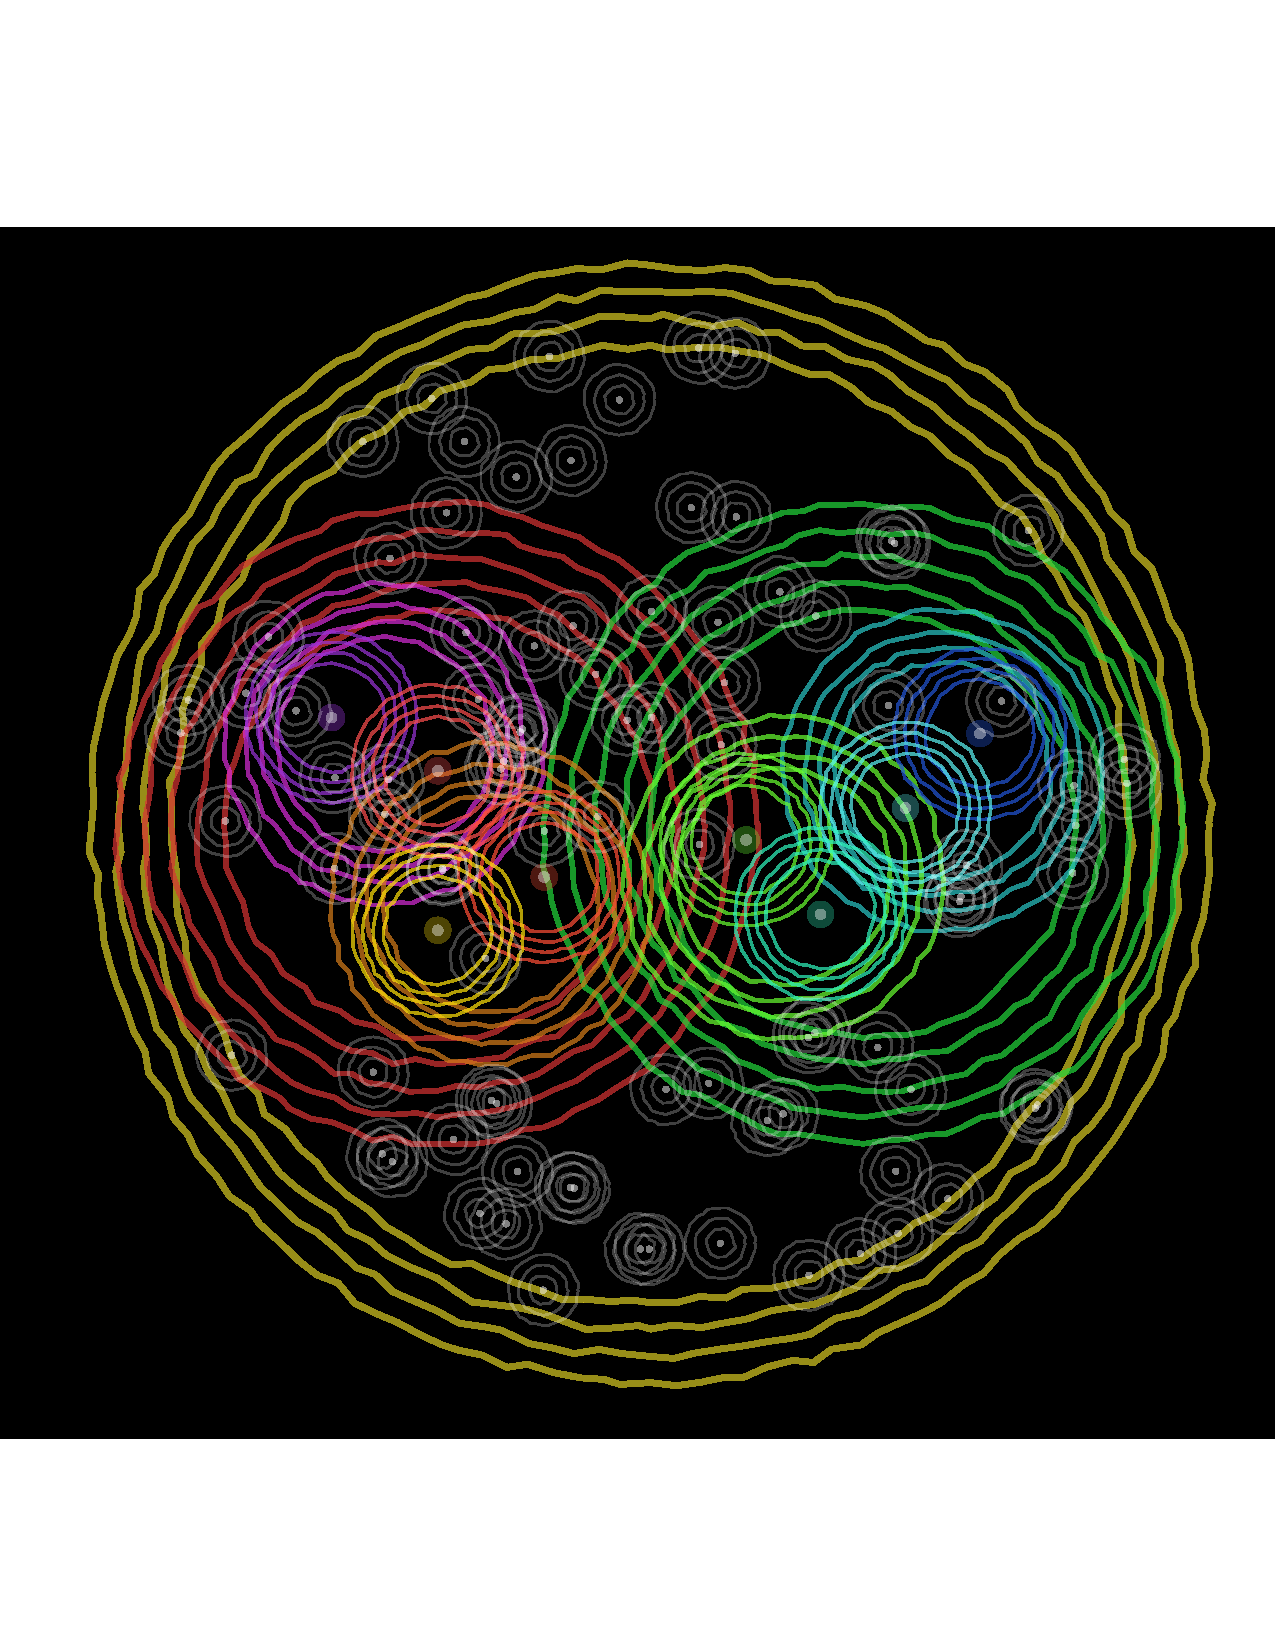
\includegraphics[width=.78\paperwidth]
                        {title/ripple}}
};
% explosion of particles
% \node[inner sep=10.1pt, outer sep=0pt](image){
%  \makebox[\textwidth]{\includegraphics[width=.80\paperwidth]
%                         {title/jettitleimage}}
% };
% \framenode[100pt]{image}
\end{tikzpicture}

% Author
\vspace{5pt}  % for ripple
\textcolor{amber}{\subtitlefont{Samuel Alipour-fard}}
\end{center}

\clearpage
\restoregeometry
\setcounter{page}{1}
